\documentclass[a4paper, 12pt]{report}		% general format

%%%% Charset
\usepackage{cmap}							% make PDF files searchable and copyable
\usepackage[utf8]{inputenc}					% accept different input encodings
\usepackage[T2A]{fontenc}					% russian font
\usepackage[russian]{babel}					% multilingual support (T2A)

%%%% Graphics
\usepackage[dvipsnames]{xcolor}			% driver-independent color extensions
\usepackage{graphicx}						% enhanced support for graphics
\usepackage{wrapfig}						% pro­duces fig­ures which text can flow around

%%%% Math
\usepackage{amsmath}						% Amer­i­can Math­e­mat­i­cal So­ci­ety (AMS) math fa­cil­i­ties
\usepackage{amsfonts}						% fonts from the AMS
\usepackage{amssymb}						% additional math symbols

%%%% Ty­po­grapy (don't forget about cm-super)
\usepackage{microtype}						% sublim­i­nal re­fine­ments to­wards ty­po­graph­i­cal per­fec­tion
\linespread{1.3}							% line spacing
\usepackage[left=2.5cm, right=1.5cm, top=2.5cm, bottom=2.5cm]{geometry}
\setlength{\parindent}{0pt}					% we don't want any paragraph indentation
\renewcommand{\chaptername}{}

%%%% Other
\usepackage{hyperref}							% ver­ba­tim with URL-sen­si­tive line breaks
%\DeclareUnicodeCharacter{00A0}{~}
\usepackage{float}

%------------------------------------------------------------------------------
\usepackage{listings}						% type­set source code list­ings

% Цвета для кода
\definecolor{string}{HTML}{101AF9}			% цвет строк в коде
\definecolor{comment}{HTML}{3F7F5F}		% цвет комментариев в коде
\definecolor{keyword}{HTML}{5F1441}		% цвет ключевых слов в коде
\definecolor{morecomment}{HTML}{8000FF}	% цвет include и других элементов в коде
\definecolor{captiontext}{HTML}{FFFFFF}	% цвет текста заголовка в коде
\definecolor{captionbk}{HTML}{999999}		% цвет фона заголовка в коде
\definecolor{bk}{HTML}{FFFFFF}				% цвет фона в коде
\definecolor{frame}{HTML}{999999}			% цвет рамки в коде

% Настройки отображения кода
\lstset{
	language=C++,							% Язык кода по умолчанию
	morekeywords={*,...},					% если хотите добавить ключевые слова, то добавляйте
	% Цвета
	keywordstyle=\color{keyword}\ttfamily\bfseries,
	stringstyle=\color{string}\ttfamily,
	commentstyle=\color{comment}\ttfamily\itshape,
	morecomment=[l][\color{morecomment}]{\#},
	% Настройки отображения
	breaklines=true,						% Перенос длинных строк
	basicstyle=\ttfamily\footnotesize,		% Шрифт для отображения кода
	backgroundcolor=\color{bk},				% Цвет фона кода
	%frame=lrb,xleftmargin=\fboxsep,xrightmargin=-\fboxsep, % Рамка, подогнанная к заголовку
	frame=tblr								% draw a frame at all sides of the code block
	rulecolor=\color{frame},				% Цвет рамки
	tabsize=2,								% tab space width
	showstringspaces=false,					% don't mark spaces in strings
	% Настройка отображения номеров строк. Если не нужно, то удалите весь блок
	numbers=left,							% Слева отображаются номера строк
	stepnumber=1,							% Каждую строку нумеровать
	numbersep=5pt,							% Отступ от кода
	numberstyle=\small\color{black},		% Стиль написания номеров строк
	% Для отображения русского языка
	extendedchars=true,
    literate=
        {Ö}{{\"O}}1                    {Ä}{{\"A}}1                    {Ü}{{\"U}}1
        {ß}{{\ss}}1                    {ü}{{\"u}}1                    {ä}{{\"a}}1
        {ö}{{\"o}}1                    {~}{{\textasciitilde}}1        {а}{{\selectfont\char224}}1
        {б}{{\selectfont\char225}}1    {в}{{\selectfont\char226}}1    {г}{{\selectfont\char227}}1
        {д}{{\selectfont\char228}}1    {е}{{\selectfont\char229}}1    {ё}{{\"e}}1
        {ж}{{\selectfont\char230}}1    {з}{{\selectfont\char231}}1    {и}{{\selectfont\char232}}1
        {й}{{\selectfont\char233}}1    {к}{{\selectfont\char234}}1    {л}{{\selectfont\char235}}1
        {м}{{\selectfont\char236}}1    {н}{{\selectfont\char237}}1    {о}{{\selectfont\char238}}1
        {п}{{\selectfont\char239}}1    {р}{{\selectfont\char240}}1    {с}{{\selectfont\char241}}1
        {т}{{\selectfont\char242}}1    {у}{{\selectfont\char243}}1    {ф}{{\selectfont\char244}}1
        {х}{{\selectfont\char245}}1    {ц}{{\selectfont\char246}}1    {ч}{{\selectfont\char247}}1
        {ш}{{\selectfont\char248}}1    {щ}{{\selectfont\char249}}1    {ъ}{{\selectfont\char250}}1
        {ы}{{\selectfont\char251}}1    {ь}{{\selectfont\char252}}1    {э}{{\selectfont\char253}}1
        {ю}{{\selectfont\char254}}1    {я}{{\selectfont\char255}}1    {А}{{\selectfont\char192}}1
        {Б}{{\selectfont\char193}}1    {В}{{\selectfont\char194}}1    {Г}{{\selectfont\char195}}1
        {Д}{{\selectfont\char196}}1    {Е}{{\selectfont\char197}}1    {Ё}{{\"E}}1
        {Ж}{{\selectfont\char198}}1    {З}{{\selectfont\char199}}1    {И}{{\selectfont\char200}}1
        {Й}{{\selectfont\char201}}1    {К}{{\selectfont\char202}}1    {Л}{{\selectfont\char203}}1
        {М}{{\selectfont\char204}}1    {Н}{{\selectfont\char205}}1    {О}{{\selectfont\char206}}1
        {П}{{\selectfont\char207}}1    {Р}{{\selectfont\char208}}1    {С}{{\selectfont\char209}}1
        {Т}{{\selectfont\char210}}1    {У}{{\selectfont\char211}}1    {Ф}{{\selectfont\char212}}1
        {Х}{{\selectfont\char213}}1    {Ц}{{\selectfont\char214}}1    {Ч}{{\selectfont\char215}}1
        {Ш}{{\selectfont\char216}}1    {Щ}{{\selectfont\char217}}1    {Ъ}{{\selectfont\char218}}1
        {Ы}{{\selectfont\char219}}1    {Ь}{{\selectfont\char220}}1    {Э}{{\selectfont\char221}}1
        {Ю}{{\selectfont\char222}}1    {Я}{{\selectfont\char223}}1    {і}{{\selectfont\char105}}1
        {ї}{{\selectfont\char168}}1    {є}{{\selectfont\char185}}1    {ґ}{{\selectfont\char160}}1
        {І}{{\selectfont\char73}}1     {Ї}{{\selectfont\char136}}1    {Є}{{\selectfont\char153}}1
        {Ґ}{{\selectfont\char128}}1
}

% Для настройки заголовка кода
\usepackage{caption}
\DeclareCaptionFont{white}{\color{сaptiontext}}
\DeclareCaptionFormat{listing}{\parbox{\linewidth}{\colorbox{сaptionbk}{\parbox{\linewidth}{#1#2#3}}\vskip-4pt}}
%\captionsetup[lstlisting]{format=listing,labelfont=white,textfont=white}
\renewcommand{\lstlistingname}{Листинг} % Переименование Listings в нужное именование структуры
\setlength{\parskip}{0.5cm}

\usepackage{pgfplots}
\pgfplotsset{compat=1.9}

%------------------------------------------------------------------------------
\begin{document}

\begin{titlepage}

%----------------------------------------------------------------------------------------
%	HEADING SECTIONS
%----------------------------------------------------------------------------------------
\begin{center} % Center everything
Федеральное государственное автономное образовательное \\
учреждение высшего образования \\[0.4cm]

\includegraphics[scale=0.8]{res/SPbPU-logo} \\[0.4cm]
Институт компьютерных наук и технологий \\*
Высшая школа интеллектуальных систем и суперкомпьютерных технологий
\end{center}

\vspace{3cm}

%----------------------------------------------------------------------------------------
%	TITLE SECTION
%----------------------------------------------------------------------------------------
\begin{center} % Center everything
\textbf{Отчёт по лабораторному практимуму N1}\\
по дисциплине "Цифровые ресурсы в научных исследованиях" \\
по теме "Распределенные реестры (блокчейн) - \\ новые концепции и технологии последних лет" \\*
\end{center}

\vspace{3cm}
 
%----------------------------------------------------------------------------------------
%	AUTHOR SECTION
%----------------------------------------------------------------------------------------
\begin{flushleft}
Выполнил студент гр. 3540901/21501 \hspace{3cm} $\underset{\text{(подпись)}}{\underline{\hspace{3cm}}}$ С.А.Мартынов\\[0.5cm]
Преподаватель \hspace{7.25cm} $\underset{\text{(подпись)}}{\underline{\hspace{3cm}}}$ Е.Н.Бендарская\\[0.5cm]
\hspace{10.2cm} «\underline{\hspace{1cm}}» \underline{\hspace{3cm}} 2022 г.
\end{flushleft}

\vfill % Fill the rest of the page with whitespace

%----------------------------------------------------------------------------------------
%	DATE SECTION
%----------------------------------------------------------------------------------------
\begin{center}
Санкт-Петербург\\
2022
\end{center}

\end{titlepage}

\setcounter{page}{2}                            % inclide the title page
\tableofcontents
%\input{text}                                 % inclide the main text
%\newpage
\section*{}
\addcontentsline{toc}{section}{List of sources}

\begin{thebibliography}{00}

% Use: \cite{label1}
\bibitem{label1} text

\end{thebibliography}                              % inclide the list of sources

\chapter*{Задание 1. Цель поиска.}
\addcontentsline{toc}{chapter}{Задание 1. Цель поиска.}

\textbf{Задание:} Определить цель поиска. Сформулировать критерии отбора информации.

\vspace{1cm}

В процессе выполнения заданий по первой работе была выявлена такая закономерность, что на русском языке наиболее релевантные запросы были получены по более общим запросам, в то время как при поиске на английском языке наблюдалась обратная ситуация. Тогда же было сделано предположение, что причина подобного феномена в неустоявшемся переводе некоторых терминов.

Для поиска на русском языке будут использоваться:
\begin{itemize}
\item "Распределённый реестр, блокчейн, консенсус, доказательство работы, доказательство владения" (поисковый запрос, включавший все поисковые слова).
\item "Распределенный реестр".
\item "Распределенные реестры (блокчейн) -- новые концепции и технологии последних лет" (поиск по названию темы аналитического отчёта).
\end{itemize}

Для поиска на английском языке будут использоваться:
\begin{itemize}
\item "Proof of stake".
\item "Proof of work".
\item "Blockchain, consensus" (комбинация двух поисковых запросов).
\end{itemize}

Так же в прошлый раз было замечено, что на английском языке было обнаружено больше материалов (в т.ч. и от исследователей из Российских университетов).

\chapter*{Задание 2. Поиск по представленным ресурсам.}
\addcontentsline{toc}{chapter}{Задание 2. Поиск по представленным ресурсам.}

\textbf{Задание}: Использовать для поиска научных статей на русском языке и английском языке представленные ниже ресурсы


Источники на русском языке
\begin{itemize}
\item \url{https://www.elibrary.ru/}
\item \url{https://www.rfbr.ru/rffi/ru/library}
\item \url{https://cyberleninka.ru/}
\item \url{http://window.edu.ru/}
\item \url{https://www.libnauka.ru/}
\item \url{http://ufn.ru/ru/}
\item \url{http://www.mathnet.ru/}
\item \url{http://www.scholar.ru/}
\item \url{https://elib.spbstu.ru/}
\end{itemize}

Источники на английском языке
\begin{itemize}
\item \url{https://link.springer.com/}
\item \url{https://nature.com}
\item \url{https://www.sciencedirect.com/}
\item \url{https://royalsociety.org/journals/}
\item \url{http://arxiv.org}
\item \url{https://core.ac.uk/}
\item \url{https://scholar.google.com/}
\item \url{https://academic.microsoft.com/}
\item \url{http://citeseerx.ist.psu.edu/}
\end{itemize}

\textbf{Результаты отбора источников представить в виде библиографического списка.}

Для систематизации набора источников использовать одну из программ для управления библиографической информацией (библиографические менеджеры), например, Mendeley.


Для управления библиографической информацией был использован библиографический менеджер Mendeley (рисунок 1). Основным затруднением является записание имён и фамилий разными стилями. Списки находятся в файлах \href{https://raw.githubusercontent.com/SemenMartynov/SPbPU_DigitalResources/main/Practice2/res/library.eng.bib}{library.eng.bib} и \href{https://raw.githubusercontent.com/SemenMartynov/SPbPU_DigitalResources/main/Practice2/res/library.rus.bib}{library.rus.bib}.

\begin{figure}[H]
 \centering
 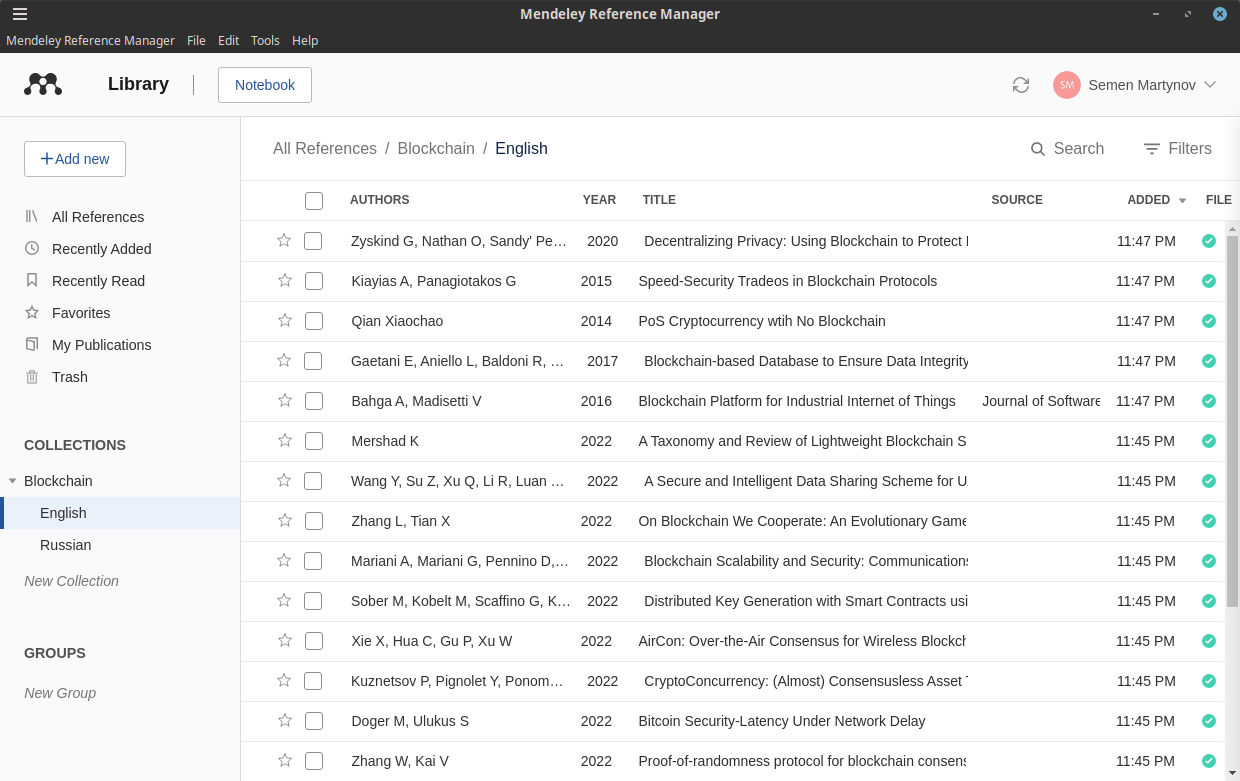
\includegraphics[scale=0.4]{res/Mendeley}
 \caption{Материалы в библиографическом менеджере Mendeley}
\end{figure}

\chapter*{Задание 3. Дополнительные научные ресурсы.}
\addcontentsline{toc}{chapter}{Задание 3. Дополнительные научные ресурсы.}

\textbf{Задание}: Дополнить список из п2. 1-2 научными ресурсами на русском и 1-2 научными ресурсами на английском языке и также провести информационный поиск.

Результаты отбора источников представить в виде библиографического списка.

\vspace{1.5cm}

Поиск дополнился сайтом \url{https://www.allcryptowhitepapers.com} и документами описывающими основные современные криптопроекты. Строго говоря, это не является научной документацией, однако ссылать на вайтпейперы ведущих проектов считается нормальной практикой.

Свежие публикации по кросс-сетевому взаимодействию удалось получить на сайте \url{https://ieeexplore.ieee.org}. Для доступа к материалам требуется пройти процедуру регистрации.

На русском языке удалось найти только сайты некоторых научных журналов, но эти материалы уже были найдены ранее через сайт \url{https://www.elibrary.ru/}.

Совершенно не научным, но достаточно интересным источником свежей информации по заданной теме является \url{https://www.twitter.com/}. В первую очередь, он позволяет отслеживать статус проектов, работа над которыми ведётся в данное время.

Дополнен файл \textit{library.eng.bib}.

\chapter*{Задание 4. Научные социальные сети.}
\addcontentsline{toc}{chapter}{Задание 4. Научные социальные сети.}

\textbf{Задание}: Дополнить результаты информационного поиска работами, найденными в научной социальной сети \url{https://www.researchgate.net/} или \url{https://www.academia.edu/}. Отметить насколько отличаются результаты поиска от п.2.

\vspace{1cm}

Сайт \url{https://www.researchgate.net/} предоставляет большой выбор свежих материалов. Многие статьи уже ранее были найдены через \url{https://www.sciencedirect.com/} и \url{http://arxiv.org}, но \url{https://www.researchgate.net/} позволяет обсудить материал с автором.

Сайт \url{https://www.academia.edu/} предложил меньше полезной информации, но он примечателен тем, что имеет готовую гистограмму, показывающую рост интереса к теме (рисунок 2 и 3).

\begin{figure}[H]
 \centering
 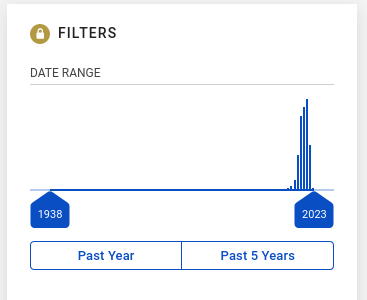
\includegraphics[scale=0.6]{res/academia1}
 \caption{academia.edu: распределение числа публикаций по запросу "Blockchain, consensus"}
\end{figure}

\begin{figure}[H]
 \centering
 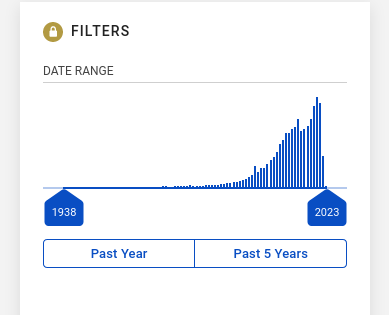
\includegraphics[scale=0.6]{res/academia2}
 \caption{academia.edu: распределение числа публикаций по запросу "Proof of work"}
\end{figure}

Дополнен файл \textit{library.eng.bib}.

\chapter*{Задание 5. Оценка удовлетворенности и достаточности.}
\addcontentsline{toc}{chapter}{Задание 5. Оценка удовлетворенности и достаточности.}

\textbf{Задание}: Оценить качество и количество полученных результатов поиска для каждого ресурса (включая дополненные самостоятельно и научных соц. сетей) -- оценка степени удовлетворенности качеством представленных источников от 1 (совсем не соответствует ожиданиям) до 10 (именно то, что ожидалось найти) и оценка достаточности представленных источников от 1 (очень мало) до 10 (очень много), а также оценить степень удобства использования для получения источников информации.

Источники на русском языке
\begin{itemize}
\item \url{https://www.elibrary.ru/} -- Удовлетворённость: 10 -- Полнота: 10
\item \url{https://www.rfbr.ru/rffi/ru/library} -- Удовлетворённость: 1 -- Полнота: 1
\item \url{https://cyberleninka.ru/} -- Удовлетворённость: 10 -- Полнота: 10
\item \url{http://window.edu.ru/} -- Удовлетворённость: 0 -- Полнота: 0
\item \url{https://www.libnauka.ru/} -- Удовлетворённость: 2 -- Полнота: 2
\item \url{http://ufn.ru/ru/} -- Удовлетворённость: 3 -- Полнота: 3
\item \url{http://www.mathnet.ru/} -- Удовлетворённость: 2 -- Полнота: 2
\item \url{http://www.scholar.ru/} -- Удовлетворённость: 1 -- Полнота: 1
\item \url{https://elib.spbstu.ru/} -- Удовлетворённость: 1 -- Полнота: 1
\end{itemize}

Источники на английском языке
\begin{itemize}
\item \url{https://link.springer.com/} -- Удовлетворённость: 8 -- Полнота: 8
\item \url{https://nature.com} -- Удовлетворённость: 4 -- Полнота: 4
\item \url{https://www.sciencedirect.com/} -- Удовлетворённость: 9 -- Полнота: 9
\item \url{https://royalsociety.org/journals/} -- Удовлетворённость: 0 -- Полнота: 0
\item \url{http://arxiv.org} -- Удовлетворённость: 10 -- Полнота: 10
\item \url{https://core.ac.uk/} -- Удовлетворённость: 5 -- Полнота: 5
\item \url{https://scholar.google.com/} -- Удовлетворённость: 10 -- Полнота: 10
\item \url{https://academic.microsoft.com/} -- Удовлетворённость: 0 -- Полнота: 0
\item \url{http://citeseerx.ist.psu.edu/} -- Удовлетворённость: 2 -- Полнота: 2
\end{itemize}

Дополнительные научные ресурсы
\begin{itemize}
\item \url{https://www.allcryptowhitepapers.com/} -- Удовлетворённость: 10 -- Полнота: 10
\item \url{https://ieeexplore.ieee.org} -- Удовлетворённость: 5 -- Полнота: 5
\item \url{https://www.twitter.com/} -- Удовлетворённость: 9 -- Полнота: 9
\end{itemize}

Научные социальные сети
\begin{itemize}
\item \url{https://www.researchgate.net/} -- Удовлетворённость: 8 -- Полнота: 8
\item \url{https://www.academia.edu/} -- Удовлетворённость: 4 -- Полнота: 4
\end{itemize}

Удовлетворённость прямо коррелирует с полнотой.


Наиболее раздражающим в плане работы была необходимость постоянно регистрироваться на разных сайтах и ожидать подтверждающего e-mail. Гораздо приятнее работать с сайтами которые сразу дают доступ к PDF без регистрации.



\chapter*{Задание 6. Гистограмма давности и численности работ.}
\addcontentsline{toc}{chapter}{Задание 6. Гистограмма давности и численности работ.}


\textbf{Задание}: Оценить давность и общее число работ. Результат представить в виде гистограммы распределения работ по годам по всему получившемуся библиографическому списку.


\begin{center}
\begin{tikzpicture}
\begin{axis}[
	ybar,
	width = 380pt,
	/pgf/number format/1000 sep={},
	legend style={
		at={(0.5,-0.25)},
		anchor=south,
		legend columns=-1
	}
]
\addplot coordinates {
	(2014,1) (2015,1) (2016,1) (2017,1) (2018,1) (2019,2) (2020,5) (2021,8) (2022,15)
};
\legend{Количество материалов опубликованных за указанный год}
\end{axis}
\end{tikzpicture}
\end{center}


Стоит отметить недостаточную чистоту выборки, т.к. я сознательно отдавал предпочтение более свежим публикациям.


\chapter*{Задание 7. Защищенные в СПбГПУ бакалаврские и магистерские работы.}
\addcontentsline{toc}{chapter}{Задание 7. Защищенные в СПбГПУ бакалаврские и магистерские работы.}


\textbf{Задание}: Найти защищенные в СПбГПУ бакалаврские и магистерские работы близкие по теме к Вашей теме \url{https://elib.spbstu.ru/}.


Привести 1-2 наиболее релевантные. Оценить давность и общее число работ.


\vspace{1cm}


Среди выпускных квалификационных работ обнаружено достаточно много материалов для изучения. Особенностью этих работ является их бОльший объём, в сравнении с ранее изученными материалами. Также обращает на себя внимание явный рост популярности темы (рисунок 4).


\begin{figure}[H]
 \centering
 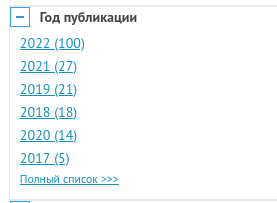
\includegraphics[scale=0.6]{res/elib}
 \caption{elib.spbstu.ru: распределение числа квалификационных работ по запросу "Блокчейн консенсус"}
\end{figure}


Также обращает на себя явно прикладной характер большинства работ. Они сделаны студентами с дипломами в области Экономики или Менеджмента. Наиболее релевантную работу привести затруднительно.


\chapter*{Задание 8. Защищенные в России кандидатские и докторские диссертации.}
\addcontentsline{toc}{chapter}{Задание 8. Защищенные в России кандидатские и докторские диссертации.}


\textbf{Задание}: Найти защищенные в России кандидатские и докторские диссертации близкие по теме к Вашей теме \url{https://search.rsl.ru/ru#ff=07.09.2020&s=fdatedesc}.


Привести 1-2 наиболее релевантные. Оценить давность и общее число работ.


\vspace{1cm}


Сайт не позволяет изучать работы так просто, как это делают другие площадки. Ссылаясь на статью 1275 Гражданского Кодекса Российский Федерации, вводится ограничение на доступ к документу.


Среди кандидатских и докторских диссертации так же выделяется тренд на повышение интереса к теме (рисунок 5). Можно заметить некоторе снижение в 2022м году, но предположу что это связано с тем, что новые данные не успели поступить в поисковую систему. И также работы прикладного характера, в первую очередь связанные с Экономикой (рисунок 6).


\begin{figure}[H]
 \centering
 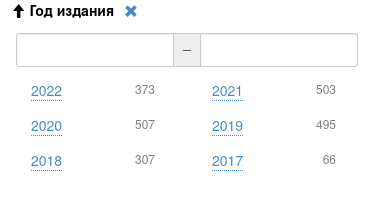
\includegraphics[scale=0.6]{res/rsl1}
 \caption{search.rsl.ru: распределение числа работ по запросу "Блокчейн консенсус"}
\end{figure}


\begin{figure}[H]
 \centering
 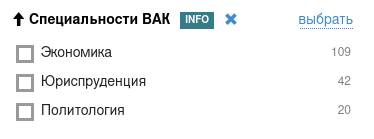
\includegraphics[scale=0.6]{res/rsl2}
 \caption{search.rsl.ru: распределение специальностей по запросу "Блокчейн консенсус"}
\end{figure}


При фильтрации по техническим наукам, я получил 4 публикации связанные с исследованиями безопасности on-chain разработки. Что не релевантно исходным запросом, т.к. я больше фокусировался на исследование алгоритмов консенсуса



\chapter*{Задание 9. Проверить наличие запатентованных РИД.}
\addcontentsline{toc}{chapter}{Задание 9. Проверить наличие запатентованных РИД.}


\textbf{Задание}: Проверить наличие запатентованных РИД (результатов интеллектуальной деятельности) по Вашей теме в системе ФИПС \url{https://new.fips.ru/iiss/} и в ресурсе, предоставляемом Яндекс \url{https://yandex.ru/patents}.


Поиск выполнить как по Российским, так и по Международным документам \url{https://new.fips.ru/about/vptb-otdelenie-vserossiyskaya-patentno-tekhnicheskaya-
biblioteka/patentnyy-poisk.php} \url{https://new.fips.ru/elektronnye-servisy/internet-resursy/index.php}.


Сравните результаты, оцените удобство поиска и релевантность, полученных документов. Оценить давность и общее число работ. Результат представить в виде гистограммы распределения работ по годам.


\vspace{1cm}


По моим ожиданиям, не должно быть большого количества патентов в исследуемой области. Это связано с тем, что разработка ведётся по большей части методом открытых исходных кодов и доверие возникает за счёт возможности публичного аудита любого кода.

Тем не менее, было обнаружено некоторое количество патентов на прикладные разработки. Примеры:
\begin{itemize}
\item RU2020666709: Программное обеспечение распределенного Реестра данных участников процесса планирования и обеспечения полетов воздушных судов (2020 г)
\item RU2021616844: Программное обеспечение реализующее логику работы узла распределенного реестра (СРР) (2021 г)
\item RU2021681494: Программное средство работы с распределенным реестром и распределенной файловой системой для организации инфраструктуры открытых ключей (2021 г)
\end{itemize}


\textbf{Поиск по Российским документам}


Поиск в системе ФИПС достаточно специфичен, в том плане что интерфейс переусложнён и ломает привычный пользовательский опыт. При поиске по всем возможным базам, было найдено 103 документа, и снова ярко выделяется тренд на практическую направленность этих документов (рисунок 7).


\begin{figure}[H]
 \centering
 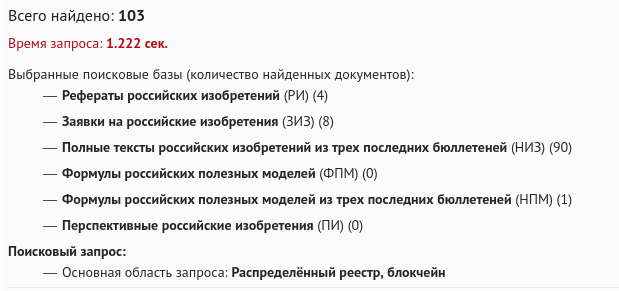
\includegraphics[scale=0.6]{res/fisp}
 \caption{fips.ru: поиск по запросу "Распределённый реестр, блокчейн"}
\end{figure}


При использовании поисковой системы Яндекс, было получено 106 документов. Очевидно, множество поисковых результатов в значительной степени пересекаются. Кроме того, Яндекс предоставляет гистограмму распределения дат документов (рисунок 8).


\begin{figure}[H]
 \centering
 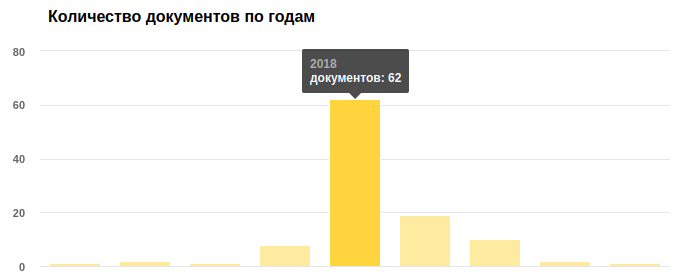
\includegraphics[scale=0.6]{res/yandex}
 \caption{yandex.ru/patents: Распределение документов по годам при поиске по запросу "Распределённый реестр, блокчейн"}
\end{figure}


При этом наблюдается нарушение тренда: до этого количество документов год от года увеличивалось, но на этом рисунке мы видим пик в 2018 году, после чего наметился спад.


\textbf{Поиск по Международным документам}


В качестве международной системы, была использована патентная БД Соединенных штатов Америки \url{https://ppubs.uspto.gov/pubwebapp/static/pages/ppubsbasic.html}. Поисковая система позволяет вводить по одному слову явно выбирая логические операции (И/ИЛИ) между ними. По запросу "Blockchain, consensus" было получено 12 494 результатов. Многие из них были опубликованы в течение последнего месяца, что говорит об актуальности данных. Доступ не требует регистрации и позволяет сразу прочитать PDF файлы. Среди недостатков можно отметить достаточно медленную работу систему -- время ожидания составляет десятки секунд, что заметно для конечного пользователя.

Другой используемой системой стала БД патентного ведомства Китая \url{english.cnipa.gov.cn}, где можно произвести поиск национальных патентных документов. Эта система требует регистрации, а интерфейс позволяет выбрать удобный язык (в т.ч. и Русский). Поисковый результат содержит 2 962 позиции, и видно за многими документами стоят крупные компании (Visa, Alipay, Microsoft). Система вполне практична для использования, но иногда подсветка найденных слов даёт сбой и ключевые слова просто игнорируются.




\chapter*{Задание 10. Поиск по базам выполненных или продолжающихся проектов.}
\addcontentsline{toc}{chapter}{Задание 10. Поиск по базам выполненных или продолжающихся проектов.}


\textbf{Задание}: Поиск по базам выполненных или продолжающихся проектов \url{https://www.rscf.ru/contests/search-projects/} и \url{https://www.rfbr.ru/rffi/ru/project_search}


Оценить давность и общее число проектов. Результат представить в виде гистограммы распределения проектов по годам.


Сайт \url{https://www.rfbr.ru} не дал никакой информации, несмотря на максимально широкий запрос.


Сайт \url{https://www.rscf.ru/} выдал 9 результатов, при максимально широких условиях запроса. Но полнота этих данных вызывает сомнения.


\begin{center}
\begin{tikzpicture}
\begin{axis}[
	ybar,
	width = 250pt,
	/pgf/number format/1000 sep={},
	legend style={
		at={(0.5,-0.25)},
		anchor=south,
		legend columns=-1
	}
]
\addplot coordinates {
	(2018,1) (2019,3) (2020,1) (2021,2) (2022,2)
};
\legend{Количество проектов, поддержанных Российским научным фондом}
\end{axis}
\end{tikzpicture}
\end{center}


\chapter*{Заключение}
\addcontentsline{toc}{chapter}{Заключение}


Из русскоязычных источников, наиболее полными и удобными являются \url{https://www.elibrary.ru/} и \url{https://cyberleninka.ru/} (тот же результат наблюдался и в первой работе). Из англоязычных -- \url{http://arxiv.org} и \url{https://scholar.google.com/}.


Об актуальном состоянии различных проектов гораздо удобнее узнавать в \url{https://twitter.ru/}, чем в более официальных источниках, подобных сайту Российского научного фонда. Помимо официальных научных источников, информацию можно получать из whitepapers развиваемых проектов.


Так же явно заметен тренд на увеличение интереса к теме за последние 3 года по значительному увеличению количества сделанных публикаций.


Многие сервисы требуют регистрацию. Это неудобно в процессе быстрого поиска информации, и создаёт риск засветить свой адрес в различных базах рассылки спама.


Библиографический менеджер Mendeley показал себя как невероятно удобное приложение, особенно при работе с англоязычными материалами, где лучше работает распознование мета-информации. Русскоязычные материалы приходится дополнительно обрабатывать руками, в частности написание имён авторов.


\end{document}

%------------------------------------------------------------------------------
% Examples:
%
%
%
% \begin{figure}[H]
% \centering
% \includegraphics[scale=0.8]{res/pic01}
% \caption{Picture description}
% \end{figure}
%
%
%
% \begin{table}[htb]
%     \begin{tabularx}{\textwidth}{|X|c|c|c|c|c|}
%     \hline
%     \multirow{2}{*}{tb1} & \multirow{2}{*}{tbl2} & \multicolumn{4}{c|}{tbl3} \\
%     \cline{3-6}
%     {} & {} & A & B & C & D\\
%     \hline
%     Text & {} & Text & {} & {} & {} \\
%     \hline
%     \end{tabularx}
% \caption{Table description}
% \end{table}